\section{Learning agents}

\begin{figure}[H]
    \centering
    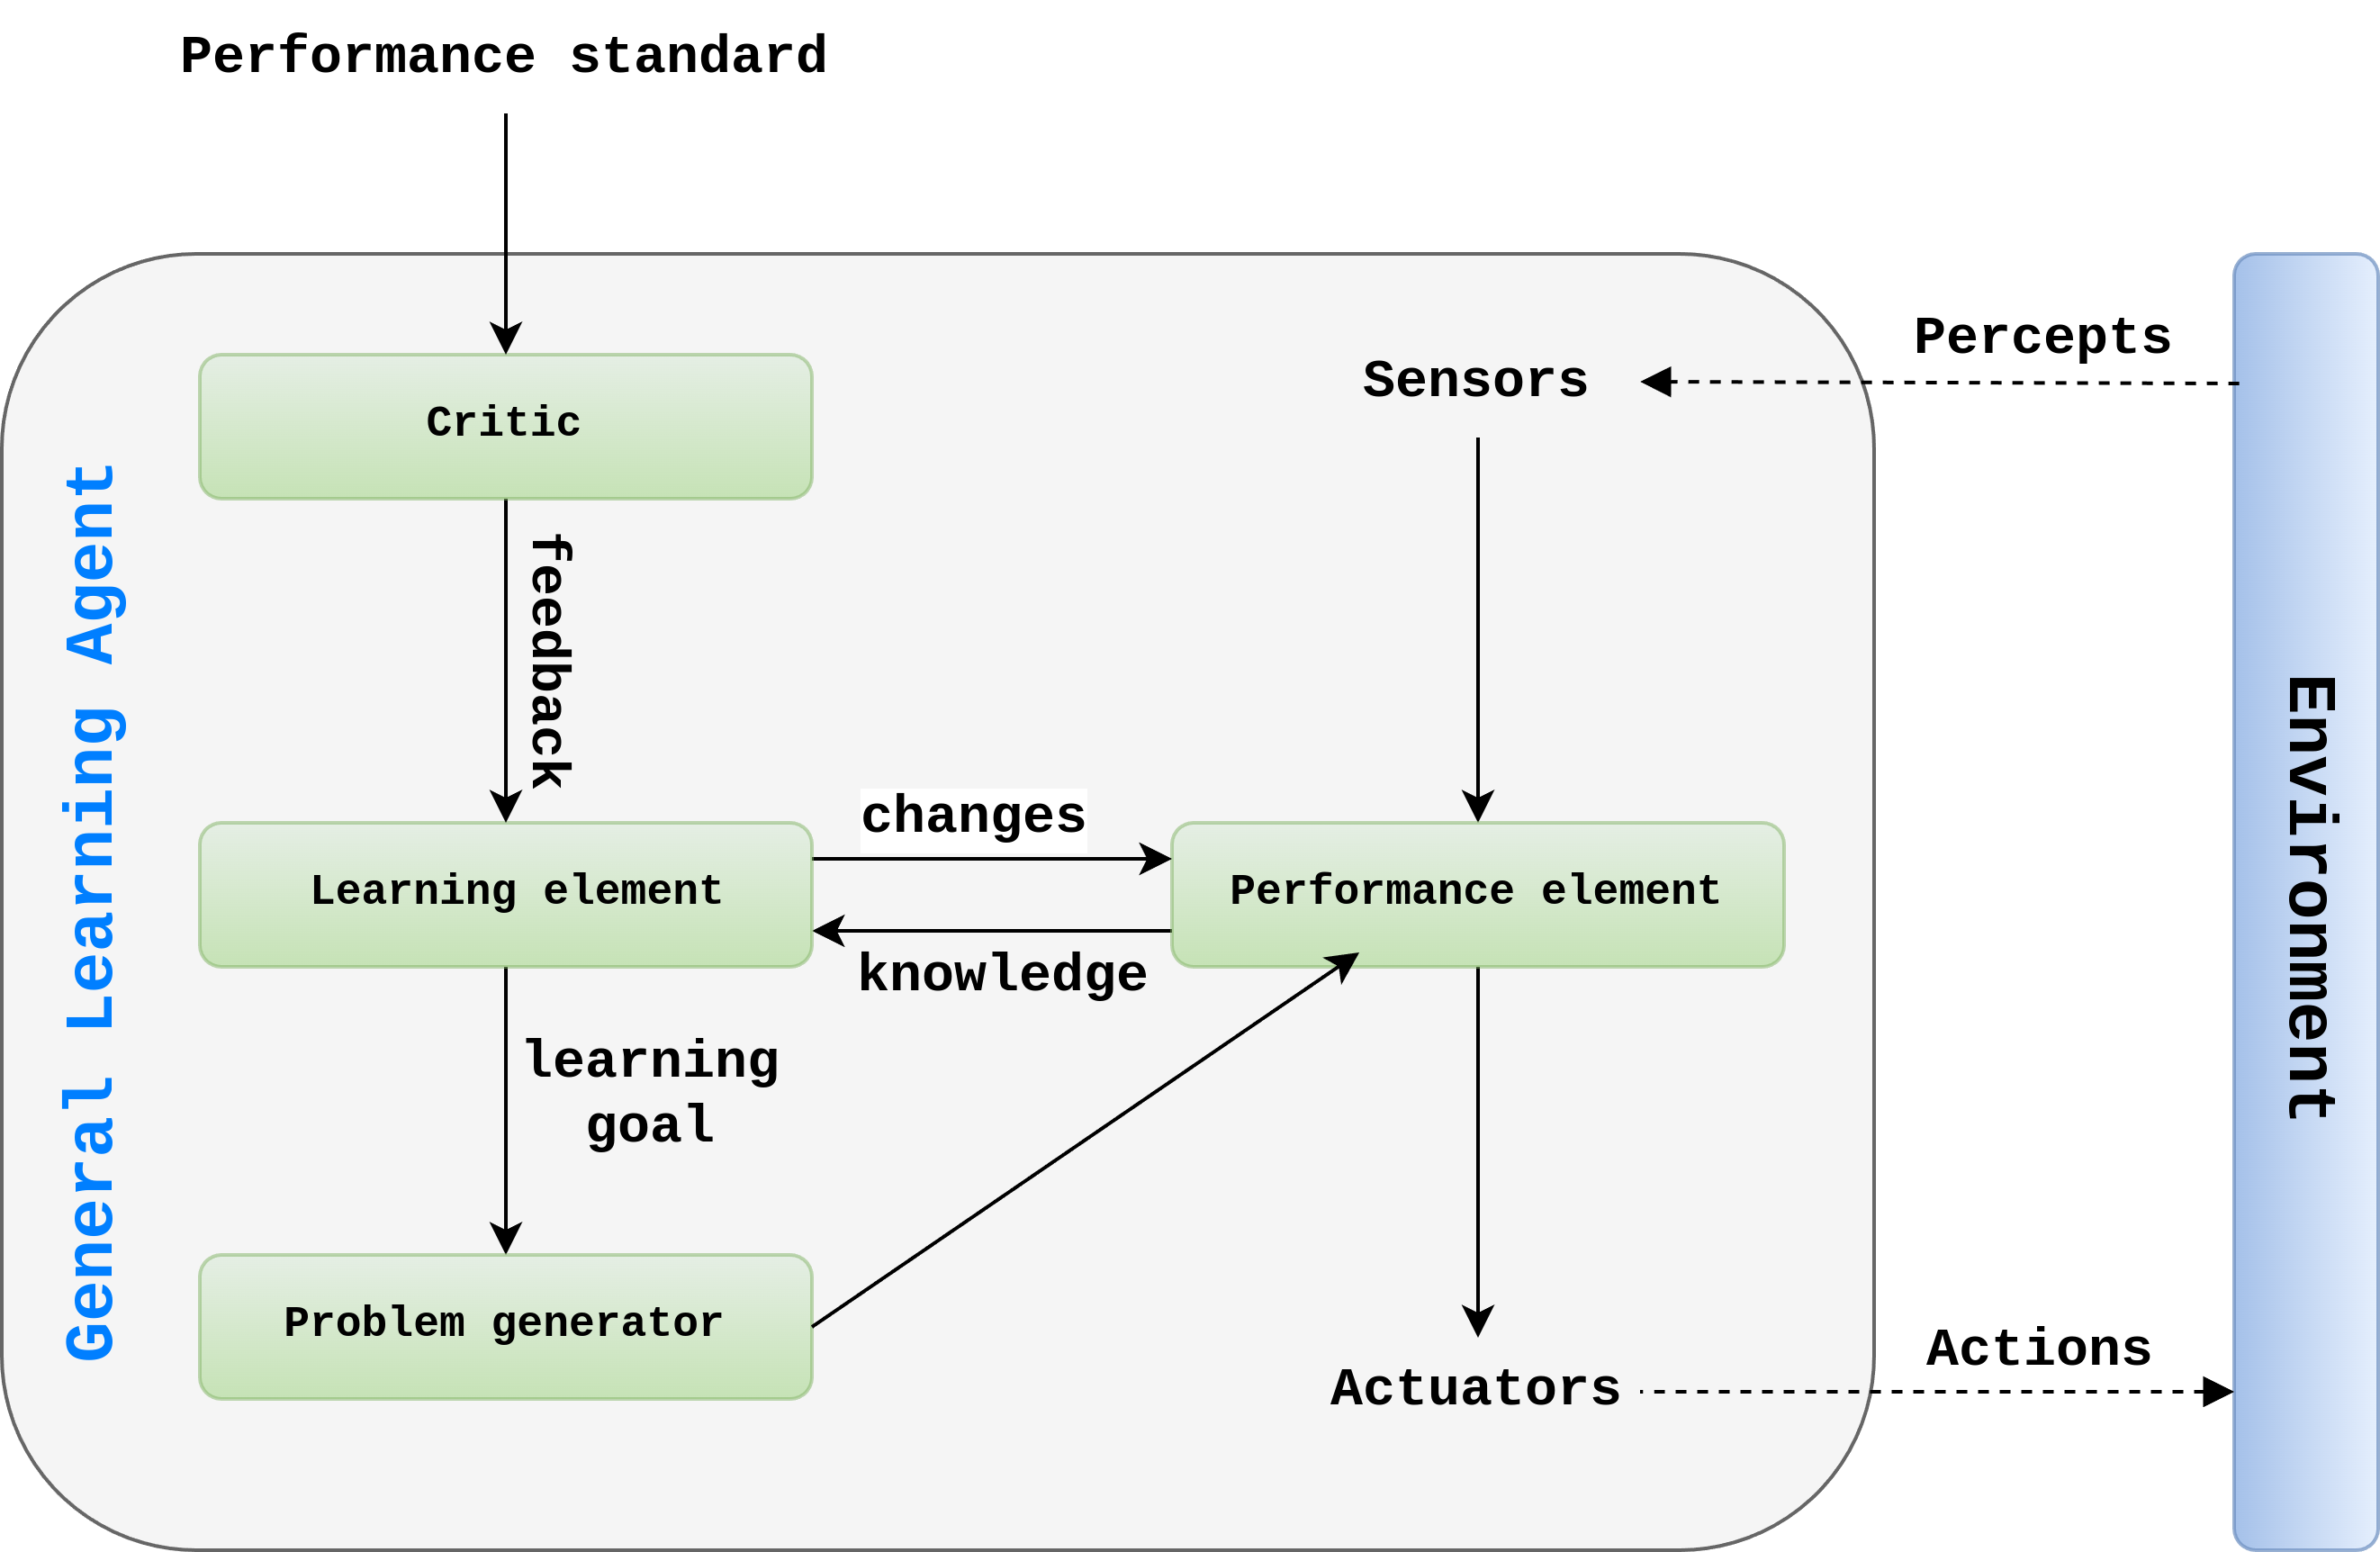
\includegraphics[
        width=0.5\linewidth, 
        height=6cm, 
        keepaspectratio
    ]{images/artificial-intelligence/ai-agents/agents-general-learning-agent.png}
    \caption*{A general learning agent. \cite{common/online/tools/draw.io}}
\end{figure}


\vspace{0.5cm}


\begin{enumerate}[itemsep=0.2cm]
    \item In his famous early paper, \textbf{Turing} (1950) considers the idea of actually programming his intelligent machines by hand.
    \hfill \cite{ai/book/Artificial-Intelligence-A-Modern-Approach/Russell-Norvig}

    \item 

\end{enumerate}


\vspace{0.5cm}




























